\chapter{Network Mobility}
\author{E. Perera, A. Seneviratne and V. Sivaraman\\
The University of New South Wales}

Providing seamless Internet connectivity to mobile hosts has been studied in
the IETF for some years now, and protocols such as Mobile IP and Mobile IPv6
have been developed. We are now witnessing the emergence of mobile networks,
namely a set of hosts that move collectively as a unit, such as on ships
aircrafts and trains. The protocols for mobility support therefore need to be
extended from supporting an individual mobile device to supporting an entire
mobile network. In this chapter the state-of-the-art in supporting the
mobility of entire networks is examined. The problem is first motivated by
considering typical network mobility scenarios and by identifying
characteristics that require new solutions. The design requirements of the
protocols that support network mobility are explored. Furthermore, current
approaches for network mobility support and their strengths and weaknesses in
addressing the design requirements is presented. The chapter is concluded by
identifying some open research issues in the realization of mobile networks.
\footnote{\copyright ACM, 2004. This is a minor revision of the work published in ACM
SIGMOBILE Mobile Computing and Communications Review, Volume 8, Issue 2 (April 2004) http:$\backslash$$\backslash$doi.acm.org$\backslash$10.1145$\backslash$997122.997127}

\section{Introduction}

The prediction that most devices will be connected to a network is fast
becoming reality with the almost ubiquitous availability of computing and
wireless communication capabilities in most electrical and electronic devices.
Two emerging forms of this ubiquitous connectedness are Personal Area Networks
(PANs) that interconnect a user's devices together and vehicle networks
especially in public transport systems which will enable groups of people to
access network services, while on the move. In such situations employing one
device namely a Mobile Router (MR) \cite{1} for the mobility management of the entire
network would be a lucrative solution in terms of performance and costs. This
architecture is advocated, in particular by the IETF's NEtwork MObility (NEMO)
Working Group \cite{2} and its popularity is evidenced by an increasing number of
commercial and research projects. The NEMO Working Group has standardized a
protocol namely NEMO Basic Support Protocol \cite{3}, that ensures uninterrupted
connectivity to nodes within a mobile network via a Mobile Router. This
protocol extends the mechanisms utilized in the host mobility management
protocol Mobile IPv6 \cite{4}.
In this chapter, the state-of-the-art for supporting network mobility is
presented by extending the survey work carried out in \cite{5}. Firstly the need for
a new network mobility architecture is motivated and then characteristics and
design goals of such an architecture is presented. This is followed by
presenting network mobility schemes in an IPv4 and IPv6 setting. Open research issues
pertaining to network mobility and some of the solutions that are proposed to
address these challenges are then discussed.

\section{Network Mobility: Why a new architecture?}

Many researchers have been working toward developing mechanisms that provide
permanent Internet connectivity to all Mobile Network Nodes (MNNs) via their
permanent IP addresses as well as maintain ongoing sessions as the mobile
network changes its point of attachment to the Internet. Host mobility
protocols such as MIP and MIPv6 are not sufficient to handle network mobility
due to two reasons. Firstly, not all devices in a mobile network such as the
sensors on an aircraft may be sophisticated enough to run these complex
protocols. Secondly, once a device has attached to the MR on a mobile network, it may not see any link-level handoffs even as the network moves. Thus the host mobility protocols such as MIP and MIPv6 do not get triggers indicating link-level handoffs and as a result will not initiate handover and would necessitate support from a MR.
NEMO Working group identifies 3 types of nodes that would be supported by a Mobile Router \cite{6}. Local Fixed Nodes, i.e., nodes which belong to the mobile network and cannot move with respect to the Mobile Router, would typically not be able to achieve global connectivity
without the support of the MR. There could also be nodes which can move with
respect to the MR namely Local Mobile Nodes (home link belongs to Mobile
network) and Visiting Mobile Nodes (home link does not belong to Mobile
network). By employing a Mobile Router to act as a gateway, all of these types of nodes within the network should be able to achieve global connectivity irrespective of their capabilities. In the following subsections, we elaborate on some of the benefits of having a network mobility architecture that relies on a Mobile Router.

\subsection{Reduced Transmission Power}

The radio transmission distance from a Mobile Network Node (such as on ships
and aircrafts) to an on-board MR is potentially much shorter than to another
Access Router on the Internet. Thus by employing the MR as an Access Router,
the nodes within the mobile network need only communicate with the MR using
minimal power and these nodes need not be equipped with specialized high-power
communication capabilities. For small devices running on battery power this
reduction in power consumption could potentially be quite significant.

\subsection{Reduced Hand-Off Signaling}

Once the Mobile Network Nodes have established a link with the MR, the link
does not need to be torn-down even as the mobile network moves. Since all
communications beyond the scope of the mobile network is via the MR, only the
MR needs to handle link layer hand-offs. This allows unsophisticated (i.e.
hand-off unaware) devices to be deployed in the mobile network, potentially
yielding low-cost mobile networks.

\subsection{Reduced Complexity}

Once a node joins a mobile network these nodes would not have to keep changing
their address since this functionality would be performed by the MR. When the mobile network changes its point of attachment to the
Internet only the MR needs to auto configure a location specific address. This
reduces the need for the Mobile Network Nodes having to perform link layer
handoffs as well as the need for auto configuring a new address. By having the
MR perform these actions on behalf of the network nodes, the software and
hardware complexity on the Mobile Network Nodes can be greatly reduced.

\subsection{Increased Manageability and scalability}

If protocol updates or additional features were to become necessary in the
future, it is much easier to update software or policies on the MR than on
each of the network nodes. Thus, a MR network mobility architecture
offers an easy central point in managing the mobility features of the entire
network and also increases the scalability of mobile networks.

\subsection{Economic Incentive}

From the point of view of transportation systems, it is often commercially
lucrative to provide and charge for global connectivity to passengers' mobile
devices through a MR installed in the vehicle, as is being currently done by
air lines.

\section{Network Mobility Characteristics and Design Requirements}

Figure 1.1 depicts a typical mobile network operational scenario of a moving
vehicle, for example an aircraft carrying passengers. The aircraft may be
equipped with various devices, such as information panels in each cabin that
provides information to the passengers, fuel sensors in the engine, and
embedded sensors that gather information such as temperature, pressure and
wind velocity. These devices together constitute the Vehicular Area Network
(VAN). Furthermore, the passengers may carry their personal wireless devices
or even an entire Personal Area Network (PAN) of devices, which enter and exit
the VAN as and when passengers embark and disembark the aircraft. A designated
node in the PAN (such as the PDA denoted in Figure 1.1 as a PAN Mobile Router --
as PMR) may act as the Mobile Router that helps connect the PAN to the VAN.
The VAN is equipped with one or more Mobile Routers designated by MR1, MR2,
and MR3 in Figure 1.1, (one MR in each cabin) that provide Internet connectivity
to the nodes within the VAN. Using the above environment as an example, in the
following sections we describe some of the characteristics of mobile networks
and discuss how they influence the protocol design. Figure 1.2 illustrates an
abstract view of a Vehicular Area Network.

\subsection{Set of Nodes Moving as a Unit}

The defining characteristic of network mobility -- the notion of a set of
nodes moving as a unit -- is evident in the above scenario. The aircraft can
be viewed as a single node changing its point of attachment to the Internet. A
network mobility protocol should be able to provide global access to all the
nodes within the mobile network.

\subsection{Local vs. Visiting Nodes}

The mobile network in the above example includes visiting nodes, such as a
passenger's wireless device, which is in a network different than its home
network, as well as local nodes, such as the information panel which is within
its home network. The network mobility protocol should cater to both these
types of nodes.

\subsection{Mobility Aware vs. Unaware Nodes}

The mobile network may contain sophisticated nodes that are \textquotedblleft
mobility aware\textquotedblright, namely, run protocols such as MIP or MIPv6
and are able to perform link layer handoffs. However, it is quite conceivable
that the mobile network may also contain nodes that are \textquotedblleft
mobility unaware\textquotedblright, that is nodes that are not sophisticated
enough to handle hand-offs. In the case of the aircraft considered above, the
temperature, pressure and wind velocity information may need to be conveyed to
a central database located outside the aircraft's network. Running
sophisticated protocols on the low-cost sensors may be infeasible, and the
network mobility support protocol should therefore be able to handle mobility
on behalf of such nodes without requiring any special support from them. This
goal, often termed \textquotedblleft Network Mobility Support
Transparency\textquotedblright, is being strongly advocated by the IETF NEMO
working group as very desirable when providing global connectivity to nodes
within a mobile network \cite{7}.

\subsection{Nested Mobility}

In the scenario considered above, the VAN of the aircraft carries within it a
PAN belonging to a passenger. Where a smaller mobile network could be
contained in a larger one is known as nested mobility. The network mobility
protocol needs to allow for at least two levels of recursive nesting.
As we shall see in a subsequent section, nested networks have implications for
routing and route optimization.

\subsection{Multi-Homed Mobile Networks}

The VAN in the aircraft shown above can be considered to be multi-homed if it
has more than one active interface connected to the global Internet -- these
interfaces could be through one MR or via the different MRs in the different
cabins. It is desirable that the Mobile Network Nodes be reachable even if one
of the active interfaces fail. It would also be desirable to allow the Mobile
Network Nodes to attach to the active interface which suits the application it
is running. For example, a passenger downloading MP3 files and listening to
music may best be supported over the least congested high bandwidth link.

It is likely that VANs, such as the aircraft VAN would use different access
technologies: satellites while flying and WLAN/UMTS whilst on the ground. A MR
offering connectivity to the nodes sitting behind it should be able to ensure
reachability to those nodes irrespective of the access technology being used.

Ernst et al \cite{8} highlights the importance of multi-homing by illustrating
the benefits and goals of multihoming considering real life scenarios.

\subsection{Different Sizes of Mobile Networks}

A passenger's Personal Area Network on its own with a single MR and few
devices such as a PDA and a mobile phone is a very small scale network. The
entire aircraft network on the other hand with a collection of subnets and a
few hundred IP devices can be categorized as a large scale network. The
network mobility solution should scale from small PANs to large VANs.

\subsection{Disparate Handoff Rates}

Wireless cells have a limited coverage area due to limited transmission range
of base stations. Mobile networks may vary significantly in the speed they
move at. For example the aircraft would be stationary or taxing at very low
speeds whilst on ground and when airborne would be moving at high speeds. In
addition the passengers themselves may be moving within the VAN. This would
result in distinct handoff frequencies and network mobility solutions have to
handle this wide range of handoffs.

\subsection{Mobile Devices from Different Administrative Domains}

A passenger's PAN could be from an entirely different domain from that of the
mobile network. The passenger's mobile devices joining the aircraft network
need to trust the MR in order to obtain Internet connectivity. This
characteristic of mobile networks which requires interaction and trust among
nodes from different domains has given rise to security issues unique to
network mobility as opposed to host mobility in a MIPv6 network. For example
Johnson et al \cite{9} eliminated the need for a local routing proxy (Foreign
Agent), which was a feature of the MIP in designing the MIPv6 protocol. This
enabled the end node to handle its own routing identifier, the Care-of
Address. In the network mobility architecture this desirable feature of MIPv6
is again compromised by having the MR as an intermediary node in the end to
end communication. This requires network mobility support solutions to address
specific security issues as well as comply with the standard IETF securities
policies and recommendations.

\section{Network Mobility in IPv4 and IPv6}

Advantages of the Mobile Router architecture have been recognized as early as
in the 1990s. Hager et al \cite{10} in their paper MINT- A Mobile Internet
Router describe of a router with sufficient computational power to perform all
necessary communication protocol operations and enable connectivity for nodes.
The MINT router provides communication software transparency and the nodes
connecting to the Internet via such a router need not be modified with basic
mobility support software. The use of a Mobile Router for network mobility has
been specified even in the very early Request For Comments \cite{11} on IP
mobility support. In the next subsections we present some of the research that
has taken place on network mobility in an IPv4 and IPv6 setting.

\subsection{IPv4 and Network Mobility}

Here we present a summary of how mobile networks are handled with the use of
IP mobility Support Protocol (MIP). This summary follows from the IP mobility
support RFC 3220 \cite{9}.

The MR would act as the foreign agent and provide a foreign agent Care-of
Address to the mobile nodes. Packets addressed to the mobile nodes within the
mobile network go through the MR's Home Agent as well as the mobile node's
Home Agent. If the nodes are fixed with respect to the mobile network then MIP
specifies two mechanisms that enable global connectivity for these nodes. One
method is to have a permanent registration with a Home Agent to reflect the
Mobile Router's home address as the fixed host's Care-of Address. Usually the
MR's Home Agent would be used for this purpose. The second method requires the
MR to advertise connectivity for the entire mobile network using normal IP
routing protocols through a bidirectional tunnel to its own Home Agent.

\subsection{IPv6 and Network Mobility}

Although it has been claimed that MIP could support mobile networks as
single mobile nodes, experimentations conducted in Motorola Planete
Inria labs \cite{12} have shown that this is not the case with the MIPv6
protocol. These experiments have shown that the Home Agent fails to redirect
packets destined for the Local Fixed Nodes sitting behind a Mobile Router. If
a packet is addressed to a Local Fixed Node the Border Router in the Home
network would attempt to forward it the MR since the MR is the next hop
towards the Local Fixed Node. The Home Agent acting on behalf of the MR
(assuming the MR has registered its new Care-of Address with the HA by means
of Binding Updates) would intercept the packet. Although the HA has a Binding
Update for the MR it has no Binding Update for the destination address on the
packet (Local Fixed Node's home address). The Home Agent being unable to
handle this packet would reroute it to the Border Router. The Border Router
would once again attempt to route this packet causing a repetition of the
above process paving the way to a routing loop. MIPv6 protocol's inability to
handle mobile networks and the network mobility characteristics and design
goals have paved the way to the NEMO Basic Support Protocol.

\subsubsection{NEMO Basic Support Protocol}

The NEMO Basic Support protocol is a natural extension to the host mobility
protocol, MIPv6. It specifies a mechanism which enables all nodes within a mobile
network to be reachable via permanent IP addresses, as well as maintain
ongoing sessions as the MR changes its point of attachment within the
topology. This protocol which runs on the MR and its Home Agent (HA) ensures
uninterrupted connectivity to the mobile network nodes, without considering
issues such as route optimization.

When a MR attaches to an Access Router in a foreign network it acquires a
Care-of Address from the visited link. Upon obtaining the new address it
informs its Home Agent of its current location by way of a registration
message, namely a Binding Update. If the MR is acting as a router as opposed
to a mobile host then this is indicated to the MR's HA by way of enabling a
the Mobile Router flag (R) in the Binding Update message. Further, the MR
informs the HA of the mobile network prefixes. (Note that in some scenarios
the Home Agent would already know which prefixes belong to a MR by
an alternate mechanism such as static configuration. In these cases, the
MR does not include any prefix information in the Binding Update.)
A positive Binding Acknowledgement from the HA with the MR flag set
received by the MR indicates the completion of the binding process and the
establishment of a bi-directional tunnel between the MR's Care-of Address and
the Home Agent's address. Any packet addressed for a Mobile Network Node would
then be intercepted by the HA and would be forwarded to the MR at its Care-of
Address. The MR, then decapsulates the packets and forwards them to the mobile
nodes. Packets in the reverse direction are also tunneled via the HA in order
to overcome Ingress filtering restrictions \cite{13}. In this case the HA
decapsulates the packets and forwards them to the Correspondent Nodes.

\paragraph{Nested Mobility Management with the NEMO protocol}

So far we have considered only Local Fixed Nodes, which are not capable of
managing their own mobility. However, a mobile node managing its own mobility
such as a passenger with a MIPv6 capable mobile device may enter the mobile
network treating it as a foreign network. Such a Visiting Mobile Node node
will send a BU to its own HA informing it to deliver all traffic to its new
Care of Address using IPv6 tunneling. This results in two, nested levels of mobility
management, since the MR manages the mobility of the mobile network. The
mobility of the Mobile Router is hidden from MNNs, even if they are capable of
handling their own mobility. Thus all packets would traverse via the Mobile
Router's Home Agent as well as the Visiting Mobile Node's Home Agent with the
NEMO protocol. This indirect routing path hinders the performance of the
Mobile Network significantly and this issue will be discussed in a subsequent section.

In the case of nested mobile networks there would be an overhead of nested
bi-directional tunnels. To illustrate the communication path and the nested
bi-directional tunnel overhead in the case of nested mobile networks, consider
a Correspondent Node (CN) that sends a packet to a mobile device in the
passenger's PAN traveling within the train's VAN. This operation of the nested
mobility scenario is depicted in Figure 1.3. Again, it is assumed that the PAN's
MR (PMR) has registered the Care-of Address it obtained from MR2, with it's HA
(HA-PMR). Furthermore as before MR2 has registered the VAN prefixes and the
Care-of Address with it's HA (HA-MR2). A packet from a CN is initially
addressed to the home address of the mobile device and gets routed to its home
network (1). In the home network it is intercepted by the HA-PMR. A route
lookup there indicates that the mobile node's prefix is at the VAN's care-of
address. The HA-PMR then encapsulates and tunnels the packet to the VAN's
care-of-address (2). At the VAN's home network this gets intercepted by VAN
Mobile Router's Home Agent HA-MR2. Its route lookup of the VAN's
care-of-address determines that the packet needs to be encapsulated and
tunneled yet again to the care-of-address in the network to which the VAN is
currently attached (3). When this doubly encapsulated packet reaches MR2,
which recognizes the outer care-of address as its own strips it off to reveal
the care-of-address of the PMR. It sends the packet to the PMR (4), which
again recognizes the (only remaining) care-of address as its own, strips it
off, and sends the original packet to the mobile device in the PAN (5).
Packets from the mobile device back to the CN traverse the same path in the
reverse direction.

\section{Network Mobility Open Research Challenges}

As described in the previous section the NEMO Basic Support protocol defines
a mechanism which enables session continuity to all Mobile Network Nodes by means of bi-directional tunneling between the MR and its HA. In defining this solution, in order to cater for mobility unaware nodes within the mobile network, the Working Group has
assumed that all nodes within the network are mobility unaware. Although this assumption guarantees complete mobility transparency to the Mobile Network Nodes it hinders the overall performance of the system significantly. This indirect routing issue and some other challenges that need to be addressed for network mobility to be a truly ubiquitous experience will be examined below.

\subsection{Indirect Routing}

According to the NEMO Basic Support protocol all packets to and from Mobile
Network Nodes traverse through the bi-directional tunnel between the MR and
its HA. This indirect routing mechanism leads to issues that degrades the
overall performance of the network. There are many undesirable side effects of
indirect routing pertaining to the NEMO protocol that have been identified
by Ng et al \cite{14}. Some of these side effects are given below.

\begin{itemize}
\item Increased packet overhead - Tunneling requires the packets to be
encapsulated thus increasing the per packet overhead. This overhead reduces
the portion of bandwidth available for application data. For example real time
traffic with a packet size of 100 bytes would experience a 40\% overhead. On a
high cost satellite link such a magnitude of overhead would not be
economically viable.

\item Increased processing delay - The encapsulation and decapsulation
processes would potentially involve tasks such as encryption/decryption which
would incur an increased processing delay.

\item Increased chances of packet fragmentation - The size of a packet
increases due to encapsulation and this could lead to potential packet
fragmentation. Packet fragmentation would result in further delays and
inefficiencies in bandwidth usage.

\item Increased susceptibility to link failure - The indirect routing creates
a longer path for each packet traversing to and from a Mobile Network Node to
Correspondent Nodes. The chances of link failure is thus higher due to the
longer path.

\item Potential bottleneck in the Home Network - Since all the packets to and
from each and every Mobile Network Node is via the Mobile Router's Home Agent,
this increased traffic load would lead to congestions at the home network.
\end{itemize}

In Figure 1.3, tracing the path from a Correspondent Node to a device in the
PAN, nested within the VAN illustrated how the route departs more and more
from the optimal as the number of nested levels increase. This multi-angular
routing issue which is referred to as pinball routing, is highly undesirable
because it amplifies the adverse effects of sub optimal routing with each
level of nested mobility. Each added level of nested mobility requires an
additional tunnel encapsulation, and these extra IPv6 headers increase the
packet size and the associated overheads. Solutions that optimize the routes
also reduce the levels of indirection, thereby overcoming the side effects of
non optimal routing such as increase in packet size. This multi-angular routing issue referred to as pinball routing could hinder the deployment of mobile networks since it gives rise to a negative impact not only on the mobile network but on the Internet as a whole.

Providing optimal routing in a network mobility setting is not an easy task.
This is due to the introduction of an intermediary node in the communication
between a node inside a mobile network and a Correspondent Node. This has
raised an issue in using MIPv6 route optimization mechanisms for network
mobility, namely that the nodes within the mobile network are unable to
perform the MIPv6 Return Routability test (RR), which is needed to
verify to the Correspondent Nodes that the home address and the Care-of
Address are collocated. Even if the Mobile Network Nodes are MIPv6 capable these nodes do not have their own Care-of Addresses, to perform route optimization. If the MR performs the MIPv6
route optimization procedure on behalf of the nodes sitting behind it, then
this would require extensions to the MIPv6 operation of Correspondent Nodes
and would also severely impact the scalability of MRs. Scalability is affected because
the MR would be required to keep account of Correspondent Nodes and would need to send Binding Updates to them on behalf of the nodes within the network. In a typical
mobility scenario such as on public transportation systems the number of
Correspondent Nodes communicating with Mobile Network Nodes could reach up to
several hundreds. Recognizing the impracticability of requiring the MR to send Binding Updates to Correspondent Nodes several route optimization solutions have been proposed and these will be presented in a subsequent section.

\subsection{Mobile Router Handoff Performance}

A NEMO handoff which is similar to a MIPv6 handoff is preceded by a link layer
handoff and an IP layer network attachment procedure. In the case of Mobile Router handoffs  Mobile Router handoffs  significant breakages in connectivity would potentially have an impact on a large number of nodes. Perera et al \cite{15} has implemented and analyzed the
handoff performance of Mobile Routers with the NEMO protocol and has shown
that the NEMO approach results in significant breakages in connectivity due to
handoffs. Their results of handoff latency \cite{16} show that due
to the NEMO handoff process all nodes within the
mobile network depending on the MR for their mobility management
incurs severe end-to-end TCP performance degradations and packet losses.

\subsection{Mobile Network Prefix Delegation}

One or more mobile network prefixes need to be assigned to a mobile network
either dynamically or statically in order for the MR to use on the links
within the mobile network. The NEMO Basic Support protocol does not provide
the means for provisioning the Mobile Routers with essential parameters such
as Home Network Prefixes. With the current NEMO protocol there is no
mechanism which enables the MR to obtain a Mobile Network Prefix
dynamically, only static configuration at the initial set up allows the MR to
obtain Mobile Network Prefixes. Static configuration could lead to binding
inconsistencies because after the initial set up of associations between the
MRs and their Mobile Network Prefixes there is no mechanism to maintain the
matching states. This could lead to routing loops and unreachable prefixes.
Further, if the Mobile Network Prefixes need to be modified there is no
mechanism to do so.

\subsection{Multihoming issues}

A multihomed mobile network would have more than one point of attachment
between the Internet and the MR. With the NEMO protocol
multihoming translates to simultaneous multiple bi-directional tunnels.
Although the NEMO Basic Support protocol neither prevents nor explicitly
specifies mechanisms to handle multihomed mobile networks there could be
issues pertaining to deploying such networks. Some of the issues pertaining to
deployment of multihomed mobile networks, as analyzed by \cite{17} is listed below.

\begin{itemize}
\item Unbroken connectivity - If one or more of the active connections fail
then there needs to be a mechanism by which the Mobile Network Nodes that were
served by the failed connection to be served by an alternate one.

\item Path Selection - In a multihomed mobile network since there would be
more than one bi-directional tunneling path available, there needs to be a
dynamic mechanism to select the most suitable path. The Home Agents, Mobile
Routers, Mobile Network Nodes and applications or a combination of these
entities should be able to select the path. In the case of a hybrid mechanism
these entities need to cooperate in making the decision.

\item Failure Detection - Failures could happen at the Mobile Routers, Home
Agents, Access Routers etc. and mechanisms to detect such
failures in time in order to make use of alternate options available in a
multihomed network would allow a more robust system.

\item Multihoming in nested mobility - There could be be many real life
scenarios where a multihomed mobile network would be nested within another
mobile network. For example in Figure 1.1 in the aircraft scenario the passenger's
PAN could potentially be a multihomed network attached to the Vehicular Area Network. Such cases of network mobility could lead to complex configurations and could possibly create infinite routing loops.
\end{itemize}

\subsection{Security and Reliability Issues}

In NEMO the MR needs to allow subscribers from different domains to get
Internet connectivity through it. In such settings where static trust
relationships are lacking a variety of security threats arise. In the NEMO
Basic Support protocol the use of IPsec to protect signaling messages is
advocated. The protocol itself does not specify any mechanisms to handle
security related or reliability related issues. Petrescu et al \cite{18} have
described the security threats related to the NEMO protocol. They have
identified signaling between the MR and the HA and nested mobility
configurations as two main sensitive points of the protocol. Jung et al
\cite{19} in their threat analysis draft on NEMO especially highlights issues
related to IPsec and other tunneling mechanisms between the MR and the HA.
Perera et al \cite{20} has identified failures of Mobile Routers in different
mobility scenarios and has shown how a new mobility architecture namely the
Ambient Networking architecture \cite{21} with its in-built enhanced failover
management functionality has a potential for creating resilient networks.
Until a new mobility architecture such as the Ambient Networking architecture
becomes a reality it is evident that security mechanisms for network mobility
would be an extremely difficult challenge.

\subsection{AAA Issues (Authentication, Authorization and Accounting Issues)}

Providing Internet access to passengers of public transportation systems would
necessitate much consideration for Authentication, Authorization and
Accounting issues. Access control is vital in such wireless public access
networks in order for any NEMO solution to be viable.

Currently within the IETF MIPv6 Working Group there is much interest shown in
adapting IPv6 AAA mechanisms for host mobility. Mechanisms to adapt the
designated AAA protocol Diameter, for a MIPv6 network is currently being
studied \cite{22}. But network mobility introduces new AAA issues due to
Mobile Network Nodes relying on a previously unknown entity to take care of
their mobility management tasks. Recognizing such issues Barz et al \cite{23}
have outlined a network access control model for vehicular mobile networks.
Since the introduction of network access control via AAA entities causes
handover delays, Barz et al \cite{23} advocate on distributing these entities
to minimize such delays.

Billing mechanisms for passengers of public transportation systems for Internet
services is a very important issue that needs to be tackled from the business
point of view.

\section{Route Optimization}

In large Mobile networks, requiring the MR to send each Correspondent Node an
individual Binding Update causes a Binding Update implosion. In order to
overcome this scalability issue Ernst et al \cite{24} have proposed a method
in which the MR sends a Prefix Scope Binding Update to a multicast address to
which Correspondent Nodes would have subscribed. A mobile network needs to
have a multicast address which it registers with the Domain Name Server (DNS).
The MR sends a periodic Binding Update containing the mobile network prefix
and the MR's Care-of Address to this multicast address. Correspondent Nodes
can join the multicast group using IPv6 multicast mechanisms. Although this
solution is beneficial for large mobile networks with many Local Fixed Nodes
it requires major changes to MIPv6 and also to the already widely deployed DNS system.

Optimized Route Cache Management protocol (ORC) \cite{25} relies on scattering
a route of a mobile network to portions of the Internet by means of Binding
Routes (an association between the mobile network prefix and the Care-of
Address) and ORC routers. Some Interior Gateway Protocol (IGP) routers named
as ORC routers are used in order to maintain a Binding Route (BR) to the
mobile network persistently. Whenever the MR moves ORC routers receives a BR
notification which will be cached in their routing tables. The ORC routers
will advertise a proxy route to the mobile network by using IGP protocols and
will capture packets destined to the mobile network. The packets will be
forwarded to the Care-of Address on the Binding Route, thus avoiding routing via the MR's
home network. Since it is not possible to make every router on the Internet an
ORC router it has been suggested that these routers be deployed in networks
where there are Correspondent Nodes for the mobile network. This scheme would
only provide optimal routing if ORC routers are available on the Correspondent
Node's networks.

Jeong et al \cite{26} proposed an optimization mechanism for MIPv6 enabled
nodes by requiring the Mobile Router to be a Neighbor Discovery proxy. This
technique requires the MR to act as bridge to the Visiting Mobile Nodes in order for these nodes to be virtually connected to the foreign link while requiring the MR to act as a router for the Local Fixed Nodes. Perera et al \cite{27} have proposed and implemented
\cite{16} a route optimization technique, OptiNets RO, which requires the MR
to act as an Access Router to the Visiting Mobile Nodes and deliver the foreign network prefix
on its Ingress interface. This enables the MIPv6 capable nodes
within the mobile network to auto configure a location specific Care-of
Address. This OptiNets RO technique exploits the desirable characteristics of
both NEMO and MIPv6 protocols. By employing this route optimization technique
it is evident that the mobile nodes need not perform a link level handoff as
in the NEMO Basic Support protocol and these nodes are able to achieve optimal
routing as in MIPv6.

Several route optimization techniques were also proposed in the context of
nested mobile networks, Kang et al \cite{28} suggested the use of a bi-directional
tunnel between the Home Agent and the Top Level MR (TLMR) to improve the routing latency. In their scheme, a tunnel is setup between TLMR of the nested mobile network and Home Agent of each MR. The TLMR advertises it's existence by using an extended Router Advertisement
message. Each MR relays the extended Router Advertisement message of TLMR
transmitted from its parent MR to it's child MR. After
receiving the extended Router Advertisement message, the MR
registers with the TLMR and notifies the address of the TLMR to it's own Home Agent. When
the  TLMR receives a registration message from the MR, it detects a
relationship between the MR and it's Access Router and uses this
information to create a tunnel to each MR. Ohnishi et al \cite{29}
proposed a HMIP-based approach for route optimization. They suggested employing
the TLMR as the MAP (as in the context of HMIPv6 \cite{30}). In
their approach, a Mobile Network Node registers it's location within the nested
mobile network once to TLMR, and also registers the location of the nested
mobile network (the TLMR's subnet address) to it's Home Agent. This
hierarchical series of registrations allows the Home Agent of MRs to directly
send packets to the TLMR.
Thubert et al \cite{31} have proposed the use of a new routing header called the Reverse
Routing Header (RRH) in order to build a nested mobile network which avoids
the nested tunnels overhead. The Reverse Routing Header which is similar to
the MIP Loose Source Routing, records the route out of the nested mobile
network. This can be converted to a routing header for packets destined to the
mobile network. In order to further illustrate the RRH solution, consider the
nested mobile network bi-directional tunneling depicted in Figure 1.3. The
packets originating from a node in the PAN has to go through two home agents
before reaching the Correspondent Node leading to very inefficient pinball
routing. If a RRH is used the PMR would in addition to tunneling the packet to
its Home Agent add a routing header with a predetermined number of slots. In
the first slot the PMR puts its home address. This packet then has the PMR's
care-of address as source address and PMR's Home Agent (HA\_PMR) as the
destination address. The next router (in this case last router) on the path
which is MR2 notices that the packet already contains a RRH, so it overwrites
the source address of the packet with its own address (MR2 care-of address)
and puts the PMR's care-of address in the second slot. The outer packet now
has MR2\_COA as source address and HA\_PMR as destination address. When the
packet reaches HA\_PMR, this Home Agent uses the information on the RRH in
entering a binding update for the PMR's home address. Now when a packet
arrives for PMR to its home network HA\_PMR can trivially construct a routing
header with MR2\_COA and PMR\_COA. This allows bypassing the home agent of
MR2. It is evident even if there are n levels of nested mobility the packet
would go through only a single Home Agent, bypassing (n-1) Home Agents.



\section{Seamless Handoffs}

A NEMO handoff can occur in two ways, 1) MR first loses connectivity with its
current Access Router and becomes unreachable at its current Care-of Address, and then
establishes connectivity with a new Access Router and acquires a new Care-of Address. This is known as a Break-Before-Make handoff. 2) MR establishes connectivity with a new AR
while still being connected to the old AR and performs a so-called
Make-Before-Break handoff after the connectivity is established. In the first
case the connectivity between MNNs and CNs is broken for the duration of the
handoff therefore the handoff latency translates directly to packet loss. In
the second case the communications are not affected by the handoff latency.

Localized mobility management schemes, such as Hierarchical Mobile IPv6 \cite{30}
and Cellular IP \cite{32} aim to reduce the effects of network latency between
Mobile Node and its Home Agent. Another large factor in Mobile IPv6 handoff
latency is the network attachment latency. Use of optimized procedures such as
Optimistic DAD \cite{33} and Fast Router Advertisements \cite{34} for the network
attachment can reduce the latency to half to two roundtrip times between
Mobile Node and its Access Router. Link layer handoffs from old base station or
Access Point to a new one and authentication procedures are another factor
affecting the handoff latency which can be improved using access technology
specific optimizations \cite{35}.

As long as a Mobile Router connects to only one network at a time and is limited
to performing Break-Before-Make handoffs, handoffs are likely to cause some
degree of disruption to traffic. Fast Mobile IPv6 \cite{36} provides an access
technology independent way of emulating Make-Before-Break handoffs by
buffering and using a localized forwarding scheme which could be used in a
network mobility setting. However, the potential performance benefits from the
emulated Make-Before-break handoffs are offset by the increased complexity
required in the access network. Petander et al \cite{37} has addressed this issue and
has proposed and implemented an access technology independent
Make-Before-Break handoff scheme for Mobile Routers. They have shown that by
using a dual interface MR where one interface is utilized for data
communications and the other interface for scanning it is possible to achieve
virtually loss free handoffs. Since the scanning and the handoff is performed
on a different interface to that of the active interface this approach enables
Make-Before-Break handoffs and minimizes the packet losses incurred due to
handoff latencies without any network infrastructure support. A further
benefit of this approach is that it alleviates the periodic interruption to
the active data communication that would occur if scanning is performed on the
same interface.

\section{Prefix Delegation Mechanisms for NEMO}

Droms et al \cite{38} has extended the DHCPv6 protocol to handle the
assignment of dynamic prefix delegation for NEMO. In order to do so they
extend the Home Agent capabilities to perform the duties of a DHCPv6
Delegating Router and the Mobile Router to perform the capabilities of a
Requesting Router. The DHCPv6 protocol messages would flow through the NEMO
bidirectional tunnel between the Home Agent and the Mobile Router. Kniveton et
al \cite{39} argues that this DHCPv6 based solution is not desirable due to
reasons such as the need for the Home Agent to have a colocated Delegating
Router functionality, operational overheads etc. Thus they advocate on
extending the NEMO Basic Support protocol in order for the MR to
synchronize its Mobile Network Prefixes and obtain new ones dynamically
instead of using another protocol such as DHCPv6 Prefix delegation protocol.
They propose extensions to the current NEMO protocol in order to handle
dynamic prefix delegation, resynchronization at binding creation after loss of
states, Mobile Network Prefix renumbering and configuration checking for loop avoidance.

\section{Multihoming Solutions}

A mobile network being multi-homed due to the MR being multi-homed is one of
the least complicated configurations. This case can be handled by the
solutions proposed for host mobility since the MR is seen as a
single node in the global topology. On the other hand much research work needs
to be done in order to handle multi-homed mobile networks due to multiple MRs.

The Inter Home Agents protocol (HAHA) proposed by Wakikawa et al \cite{40}
allows a Mobile Router/Mobile Node to utilize multiple Home Agents
simultaneously. The adopted mechanism is to place multiple Home Agents serving
the same home prefix on different links which coordinate with each other to
provide Home Agent redundancy and load balancing. Chung et al \cite{41} addresses the
issue of, how to "best" distribute the user traffic among the set of available
access networks in a multihomed on-board mobile network. Two traffic
distribution schemes are proposed which optimizes the profit and performance
of the mobile network operator. In order for policy driven mechanisms
supported by multi-homed mobile networks to be realized it is necessary to
consider accounting issues that arise inadvertently. Providing QoS for mobile
network nodes by exploiting the redundancy provided in multi-homed mobile
networks is a research area that needs further study.

\section{Network Mobility Projects}

Along with the IETF NEMO working group network mobility research projects
influences the evolvement of network mobility protocols. We consider some of
these projects in the following subsections.

\subsection{eMotion (Network in Motion) child project of OCEAN (On-board
Communication, Entertainment And iNformation)}

OCEAN \cite{42} which is a University of New South Wales and Australian
Research Council sponsored project with collaborators being National ICT
Australia (NICTA) \cite{43} and Boeing Airline Company was founded in 2003.
This project recognizes the need for extension of Internet services for public
transportation systems and encompasses two research areas namely networking
and data management. The child project eMotion \cite{44} handles networking
issues pertaining to providing global Internet access to passengers via Mobile
Routers and wide area wireless access systems. This project has implemented a
network mobility test bed \cite{45} and has studied the NEMO protocol extensively and
has proposed many optimizations for network mobility \cite{16}.

\subsection{Ambient Networks Project}

AMBIENT networking project \cite{21} is geared towards increasing competition and cooperation in an environment populated by a multitude of user devices, wireless technologies, network operators and business entities. This architecture aims to extend all IP networks with three fundamental requirements of today's networking world. These requirements include dynamic network composition, mobility and heterogeneity.  By encompassing these notions the Ambient Networks (AN) project strives to achieve horizontally structured mobile systems that offer common control functions to a wide range of different applications and air interface technologies. The ambient networking approach includes the flexibility of every end system to be not just a node but also an entire network. Therefore network mobility is inadvertently a central focus of this architecture.

\subsection{OverDRiVE (Over Dynamic multi-Radio networks in Vehicular
Environments)}

OverDRiVE \cite{46} is an Information Society Technologies (IST) project and
is ongoing work of the DRiVE \cite{47} project. The main objective of this
project is to enable high-quality wireless communication to vehicular networks
in multi-radio access environments. This project too uses the Mobile Router architecture for network mobility in an IPv6 setting.

\subsection{Nautilus6 (WIDE Project)}

The WIDE (Widely Integrated Distributed Environment) project which was
launched in 1988 established the Nautilus6 working group \cite{49} to deploy
mobile Internet. In order to do so the Nautilus6 Working Group uses the IETF
standards whenever appropriate. Nautilus6 NEMO working group was established
in November 2003 and is specifically looking at issues concerned with mobile
networks. This group has a demonstration test bed as well as a indoor
NEMO test bed.

\subsection{InternetCAR (Internet Connected Automobile Researches )}

The demand for Intelligent Transportation Systems (ITS) has influenced the
need for projects such as the InternetCAR \cite{50}. This project which is
also a WIDE project was launched in 1996. Their main aim is to view a car as a
node on the Internet and to provide Internet connectivity permanently and in a
transparent manner regardless of the underlying access medium.

The InternetCAR project implemented the Prefix Scoped Binding Update approach
for network mobility proposed by Ernst et al \cite{51}. The details of this
implementation and the requirements for connecting vehicles to the Internet
are described in \cite{52}.

\subsection{FleetNet - Internet On the Road}

FleetNet \cite{53} project too aims to connect vehicles to the Internet. But
the MR-HA bidirectional tunneling architecture for network mobility is not the
approach adapted when providing Internet connectivity to the devices in a
vehicle in FleetNet. This project has introduced a novel network mobility
architecture named as MOCCA (MObile CommuniCation Architecture).

The MOCCA architecture relies on a new entity namely an Internet Gateway
installed on roadsides which plays the role of a gateway router for the
devices requiring Internet connectivity. These gateways can be regarded as
FleetNet radio nodes since they run the same communication system employed on
the vehicles. The Internet Gateways have another interface which connects them
to the Internet. The devices in the vehicles are able to obtain connectivity
through the Internet Gateways transparently. This MOCCA architecture has been
developed by Bechler et al \cite{54}.

\section{Conclusion}

This chapter presented the basic network mobility architecture using mobility
scenarios in order to highlight the benefits of such an architecture. As
shown, providing basic network mobility support is relatively simple and
requires only minimal extensions to the MIPv6 operations of the MR and its
Home Agent. On the other hand, providing route optimization for the nodes
within the mobile network is quite challenging, given the MR-HA Bi-directional
tunneling architecture. The IETF NEMO working group is chartered only to
standardize solutions for basic network mobility; nevertheless numerous
members within the community are currently working on optimal routing
solutions for a network mobility setting. The future of network mobility at IP
level at a large scale relies on the ability to provide advanced mobility
support that can coexist with the currently deployed protocols.

\begin{thebibliography}{99}

\bibitem {1}J. Manner and M. Kojo, "Mobility Related
Terminology", RFC 3753, IETF, June 2004.

\bibitem {2}http://www.ietf.org/html.charters/nemo-charter.html

\bibitem {3}
V. Devarapalli, R. Wakikawa, A. Petrescu, P. Thubert, "Network
Mobility (NEMO) Basic Support Protocol", RFC 3963, IETF, January
2005.

\bibitem {4}
D. Johnson, C. Perkins and J. Arkko, "Mobility Support in IPv6", RFC
3775, IETF, June 2004.

\bibitem {5}
E. Perera, V. Sivaraman and A. Seneviratne, "Survey on Network
Mobility Support", ACM SIGMOBILE Mobile Computing and Communications
Review, Volume 8 , Issue 2, April 2004.

\bibitem {6}
T. Ernst and H-Y. Lach, "Network Mobility Support Terminology",
(draft-ietf-nemo-terminology-01), Internet Draft, IETF, February
2004, Work in Progress.

\bibitem {7}
T. Ernst, "Network Mobility Support Goals and
Requirements",(draft-ietf-nemo-requirements-04.txt), IETF, Internet
Draft, Feb. 2005, Work in Progress.

\bibitem {8}
T. Ernst, N. Montavont, R. Wakikawa, E. Paik, C. Ng, K. Kuladinithi
, T. Noel, "Goals and Benefits of Multihoming",
(draft-multihoming-generic-goals-and-benefits-01), IETF, Internet
Draft, Feb. 2005.

\bibitem {9}
C. Perkins, "IP Mobility support for IPv4,"\ RFC 3220, IETF, January
2002.

\bibitem {10}
R. Hager, A. Klemets, G. Q. Maguire, "MINT- A Mobile Internet
Router", 1st International Symposium on Global Data
Networking,Cairo, Egypt, Dec. 13-15, 1993.

\bibitem {11}
C. Perkins, "IP Mobility support for IPv4,"\ RFC 2002, IETF, October
1996.

\bibitem {12}
T. Ernst, "Network Mobiltiy Support in IPv6", Phd Thesis, University
Joseph Fourier Grenoble, France, October 2001.

\bibitem {13}
P. Ferguson and D. Senie, "Network Ingress Filtering : Defeating
Denial of Service Attacks which Employ IP Source Address Spoofing",
RFC 2267, IETF, January 1998.

\bibitem {14}
C. Ng, P. Thubert, M. Watari and F. Zhao, "Route Optimization
Problem Statement", (draft-ietf-nemo-ro-problem-statement-02),
Internet Draft, IETF, Dec., 2005, Work in Progress.

\bibitem {15}
E. Perera, H. Petander, K. Lan, A. Seneviratne, "Implementation and
Evaluation of a Mobile Hotspot", The Third ACM\ International
Workshop on Wireless Mobile Applications and Services on WLAN\
Hotspots 2005, Cologne, Germany, Sep. 2005.

\bibitem {16}
H. Petander, E. Perera, K. Lan and A. Seneviratne, "Measuring and
improving performance of network mobility management in IPv6
networks", NICTA Technical Report,
http://nicta.com.au/director/research/publications/technical\_reports/2005.cfm

\bibitem {17}
C. Ng, E. Paik, T. Ernst, "Analysis of Multihoming in Network
Mobility Support", (draft-ietf-nemo-multihoming-issues-02), Internet
Draft, IETF, Feb., 2005, Work in Progress.

\bibitem {18}
A. Petrescu, A. Olivereau, C. Janneteau, Lach H-Y., "Threats for
Basic Network Mobiltiy Support (NEMO threats)",
(draft-petrescu-nemo-threats-01.txt), IETF, Internet Draft, January
2004, Work in Progress.

\bibitem {19}
S. Jung, F. Zhao, F. Wu, H. Kim, S. Sohn, "Threat Analysis for NEMO
Basic Operations", (draft-jung-nemo-threat-analysis-02.txt),
Internet Draft, IETF, Feb. 2004, Work in Progress.

\bibitem {20}
E. Perera, A. Seneviratne, "Failover for Mobile Routers: A Vision of
Resilient Ambience", IEEE International Conference on Networking
(ICN'05), Reunion Island, April 2005.

\bibitem {21}
Ambient Networks: http://www.ambient-networks.org/

\bibitem {22}
S. Faccin,"Mobile IPv6 Authentication, Authorization and Accounting
Requirements", (draft-le-aaa-mipv6-requirements-02.txt), Internet
Draft, IETF, April 2003, Work in Progress.

\bibitem {23}
C. Barz "Network Access Control in OverDRIVE Mobile Networks", IST
Mobile Summit 2003, Aveiro, Portugal, 16-18 June 2003.

\bibitem {24}
T. Ernst, "Extending Mobile-IPv6 with Multicast to support mobile
networks in IPv6", ECUMN'00, Colmar, France, October 2-4 2000.

\bibitem {25}
R. Wakikawa, "ORC: Optimized Route Cache Management Protocol for
Network Mobility", Proceedings of the 10th Interantional Conference
on Telecommunication (ICT), Tahiti Papeete, French Polynesia, Feb
2003.

\bibitem {26}
Jaehoon Jeong, Kyeongjin Lee, Jungsoo Park and Hyoungjun Kim,
"Route Optimization based on ND-Proxy for Mobile Nodes in IPv6
Mobile Networks", IEEE VTC 2004-Spring, Milan, Italy, May 17-19,
2004.

\bibitem {27}
E. Perera, "OptiNets: An architecture to enable optimal routing for
network mobility ", International Workshop on Wireless Ad-hoc
Networks 2004 (IWWAN 2004), Oulu, Finland, 31 May -3 June, 2004.

\bibitem {28}
H. Kang, "Route Optimization for mobile network by using
bi-directional between Home Agent and Top Level Mobile Router "
(draft-hkang-nemo-ro-tlmr-00.txt), Internet Draft, IETF, June 2003.

\bibitem {29}
H. Ohnishi, "Route HMIPv6 based route optimization method in a
mobile network, " (draft-ohnishinemo- ro-hmip-00.txt), Oct. 2003.

\bibitem {30}
H. Soliman, "Hierarchical Mobile IPv6 Mobility Management (HMIPv6)
,"\ RFC 4140, IETF, Aug. 2005.

\bibitem {31}
P. Thubert, "IPv6 Reverse Routing Header and its application to
Mobile Networks",
(draft-thubert-nemo-reverse-routing-header-05.txt), Internet Draft,
IETF, June 2004, Work in Progress.

\bibitem {32}
A. Valko, "Cellular IP: a new approach to Internet host mobility",
ACM SIGCOMM Computer Communication Review, Volume 29, Issue 1,
January 1999.

\bibitem {33}
N. Moore, "Optimistic Duplicate Address Detection for IPv6, "
(draft-ietf-ipv6-optimistic-dad-05.txt), Feb. 2005.

\bibitem {34}
J. Kempf, "IPv6 Fast Router Advertisement",
(draft-mkhalil-ipv6-fastra-05.txt ), Jan. 2005.

\bibitem {35}
I. Ramani and S. Savage, "Syncscan : Practical fast handoff for
802.11 infrastructure networks", in Proceedings of IEEE INFOCOM,
Miami, Florida, Mar. 2005.

\bibitem {36}
R. Koodli, "Fast Handovers for Mobile IPv6"\ ,
(draft-ietf-mobileip-fast-mipv6-07.txt), Internet Draft, IETF,
September 19 2003, Work in Progress.

\bibitem {37}
H. Petander, E. Perera and A. Seneviratne, "Multiple Interface
Handoffs: A Practical Method for Access Technology Independent
Make-Before-Break Handoffs", NICTA Technical Report,
http://nicta.com.au/director/research/publications/technical\_reports/2005.cfm

\bibitem {38}
R. Droms, "DHCPv6 Prefix Delegation for NEMO",
(draft-ietf-nemo-dhcpv6-pd-00.txt), Internet Draft, IETF, Aug. 2004,
Work in Progress.

\bibitem {39}
T. Kniveton" Mobile Network Prefix Delegation ",
(draft-ietf-nemo-prefix-delegation-00.txt), Internet Draft, IETF,
Aug. 2005, Work in Progress.

\bibitem {40}
R. Wakikawa, "Inter Home Agents Protocol (HAHA)",
(draft-wakikawa-mip6-nemo-haha-01.txt), Internet Draft, IETF, Feb.
2004, Work in Progress.

\bibitem {41}
A. Chung and H. Mahbub, "Traffic distribution algorithm for
multi-homed mobile hotspots ", in Proceedings of IEEE Vehicular
Technology Conference (VTC),Stockholm, Sweden, Spring 2005.

\bibitem {42}http://www.ocean.cse.unsw.edu.au/

\bibitem {43}http://www.nicta.com.au/

\bibitem {44}http://www.ocean.cse.unsw.edu.au/emotion/index.html

\bibitem {45}
K. Lan, "MOBNET: The Design and Implementation of a Network Mobility
Testbed for NEMO protocol", 14th IEEE Workshop on Local and
Metropolitan Area Networks, September 18-21, 2005, Crete, Greece.

\bibitem {46}OverDRiVE: http://www.ist-overdrive.org

\bibitem {47}DRiVE : http://www.ist-drive.org/index2.html

\bibitem {48}
M. Ronai, "Mobility Issues inOverDRIVE Mobile Networks", IST Mobile
Summit 2003, Aveiro, Portugal, 16-18 June 2003.

\bibitem {49}http://www.nautilus6.org/

\bibitem {50}InternetCAR: http://www.sfc.wide.ad.jp/InternetCAR/

\bibitem {51}
T. Ernst, "Mobile Networks Support in Mobile IPv6" \
(draft-ernst-mobileip-v6-network-03) Internet Draft, IETF, March
2002, Work in Progress.

\bibitem {52}
T. Ernst, K. Mitsuya and K. Uehara, "Network Mobility from the
InternetCAR perspective", Journal Of Interconnection Networks
(JOIN), June 2003.

\bibitem {53}FleetNet : http://www.fleetnet.de/

\bibitem {54}
M. Bechler, J. Franz and L. Wolf, "Mobile Internet Access in
FleetNet", 13. Fachtagung Kommunikation in Verteilten Systemen (KiVS
2003), Leipzig, February 2003.

\end{thebibliography}

\clearpage

\begin{figure}
    \centering
        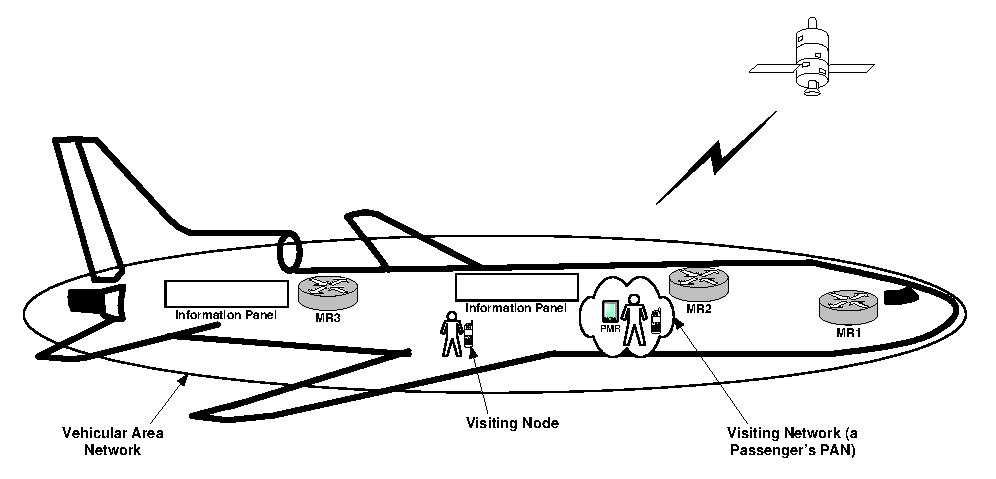
\includegraphics{Chapter1/Fig001.eps}
    \caption{Mobile Network Scenario}
    \label{fig:Fig1}
\end{figure}

\begin{figure}
    \centering
        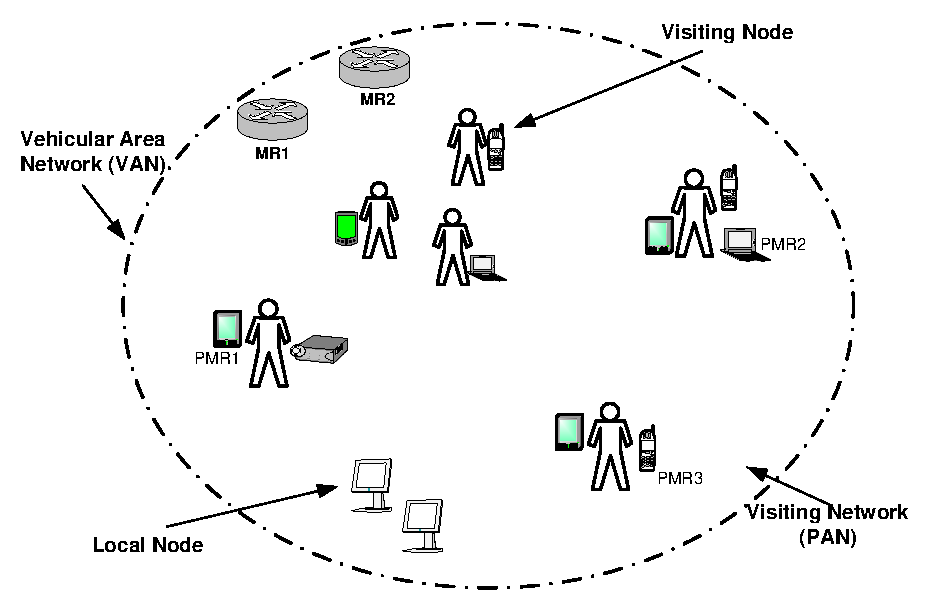
\includegraphics{Chapter1/Fig002.eps}
    \caption{Abstract View of a Vehicular Area Network}
    \label{fig:Fig2}
\end{figure}

\begin{figure}
    \centering
        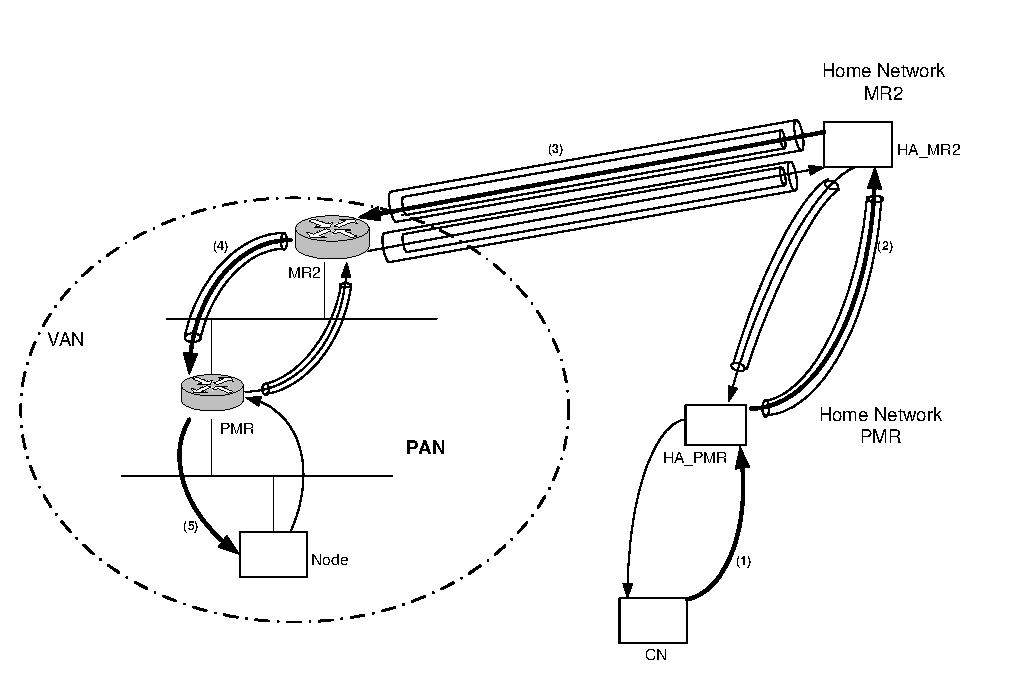
\includegraphics{Chapter1/Fig003.eps}
    \caption{Nested Bi-directional Tunneling}
    \label{fig:Fig3}
\end{figure}
